If you haven't downloaded and unzipped \href{https://libaoj.in/courses/2021f/MATH3341/zip/Math.3341.zip}{\texttt{Math.3341.zip}}. Download and unzip it under \verb|H:| (H Drive if you are working on the Remote Lab). Change the current working directory by typing \verb|cd H:\Math.3341\Math.3341.Lab.14| in the Command Window, and type \verb|edit lab_14_script| in the Command Window to edit \verb|lab_14_script.m|.

%---------------------------------------------
\section{Direction Fields and Solution Curves}
%---------------------------------------------
Given the following ODE and the initial condition,
$$
\frac{dy}{dt} = -y - 5 e^{-t} \sin(5t), \quad y(0) = -2, \quad t \in [0, 3].
$$
\begin{enumerate}[(a)]
    \item Define anoymous function \verb`dydt` to be the right-hand side of the ODE.
    \item Define \verb`a`, \verb`b` to be the left and right endpoint of the interval $[0, 3]$, respectively.
    \item Define \verb`t_step` to be the step size $\Delta t = 0.01$.
    \item Define \verb`t_span` to be a vector starting from \verb`a` to \verb`b` with step size \verb`t_step` using colon notation.
    \item Use \verb`ode23` to solve the ODE.
    \item Plot \verb`y_sol(:, i)` versus \verb`t_sol(:, i)` with line style specified in the cell array \verb`LineStyle`.
    \item Run the script and see whether it works. If it does work, add more initial conditions to \verb|y0|: $y(0) = 0$, $y(0) = 2$, $y(0) = 4$.
\end{enumerate}
%---------------------------------------------
\section{System of ODEs}
%---------------------------------------------
Next, use the built-in ODE solver \verb`ode45` to solve the following system of ODEs:
$$
\begin{cases}
    y'_1(t) = y_3, \\
    y'_2(t) = y_4, \\
    y'_3(t) = -2 y_1 + (3/2) y_2, \\
    y'_4(t) = (4/3) y_1 - 3 y_2, \\
\end{cases}
\quad
\mathbf{y}(0) =
\begin{bmatrix}
    -1 \\ 4 \\ 1 \\ 1
\end{bmatrix},
\quad
t \in [0, 15].
$$
\begin{enumerate}[(a)]
    \item Define an anoymous function (you can refer to the example in reference page for \verb`ode45`. To open the reference page, type \verb`doc ode45` in the Command Window).
    \item Repeat the steps in Part 1 to define \verb`a`, \verb`b`, \verb`t_step`, \verb`t_span`, and \verb`y0`.
    \item Use \verb`ode45` to solve the system of ODEs.
    \item Plot \verb`y(:, i)` versus \verb`t` with line style specified in the cell array \verb`LineStyle`.
    \item Plot \verb`y(:, 3)` versus \verb`y(:, 1)`.
\end{enumerate}
%---------------------------------------------
At last, run the script \verb|lab_14_script.m|. Upload the script file \verb|lab_14_script.m|, and figure files \verb|lab_14_figure_1.pdf|, \verb|lab_14_figure_2.pdf|, \verb|lab_14_figure_3.pdf| to Overleaf. Recompile, and submit the generated .pdf file on WyoCourses.

\begin{figure}[!hbtp]
  \centering
  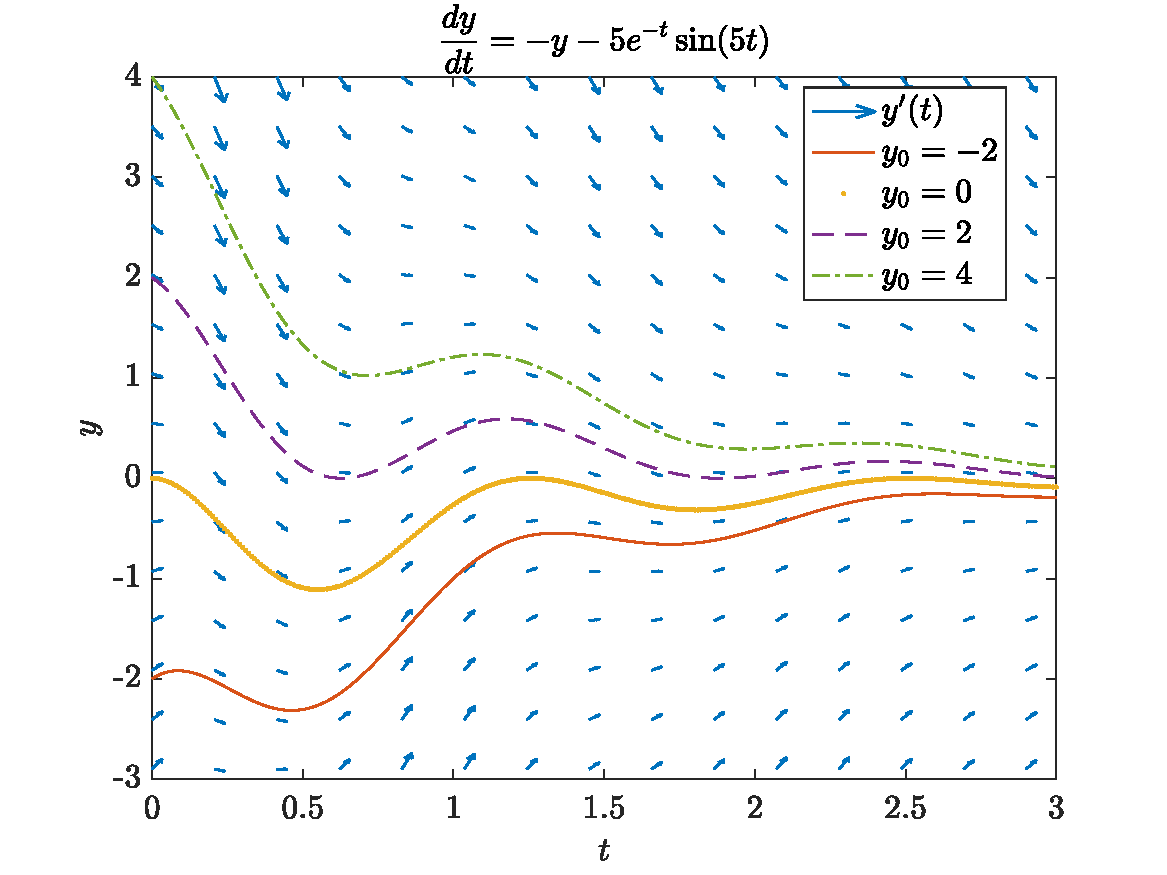
\includegraphics[height=0.3\textheight]{../Math.3341.Lab.14.ans/lab_14_figure_1.pdf}
  \caption{Expected result for Direction Fields and Solution Curves}
  \label{fig:}
\end{figure}

\begin{figure}[!hbtp]
  \centering
  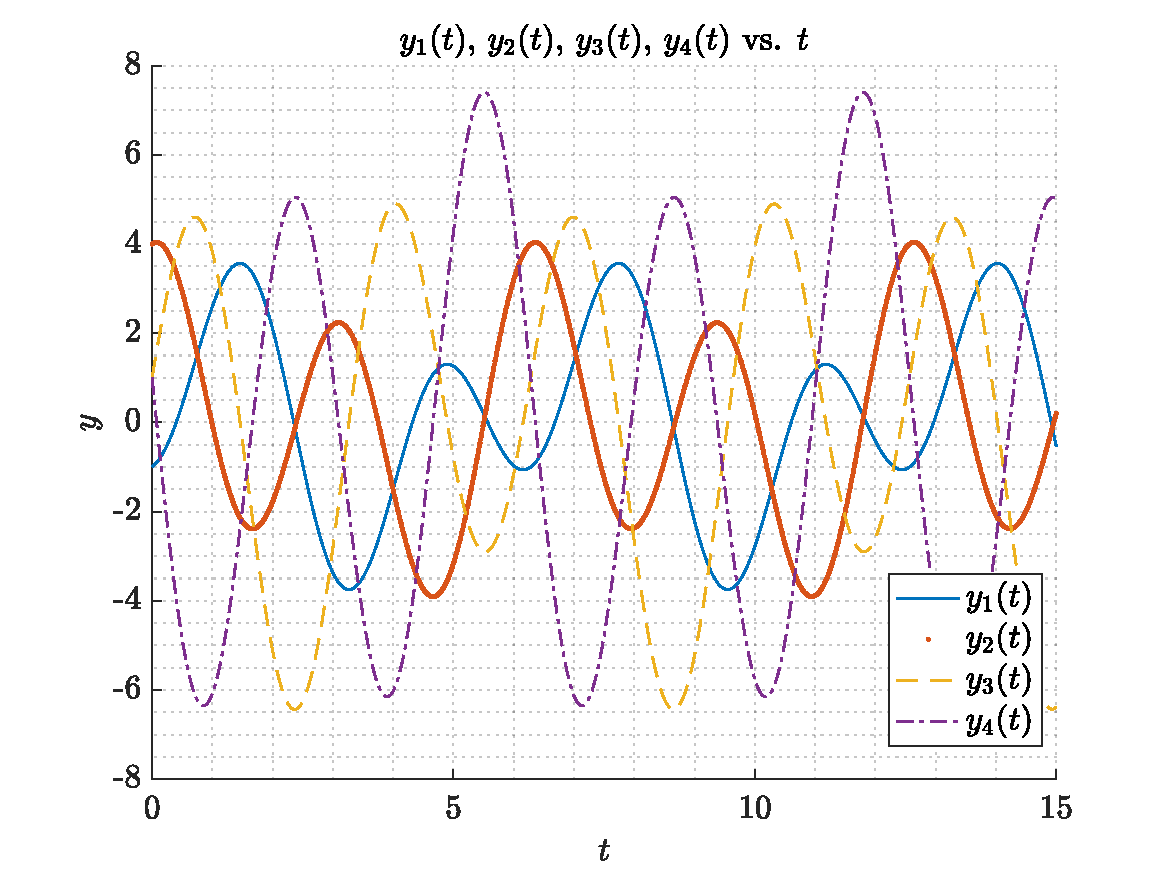
\includegraphics[height=0.3\textheight]{../Math.3341.Lab.14.ans/lab_14_figure_2.pdf}
  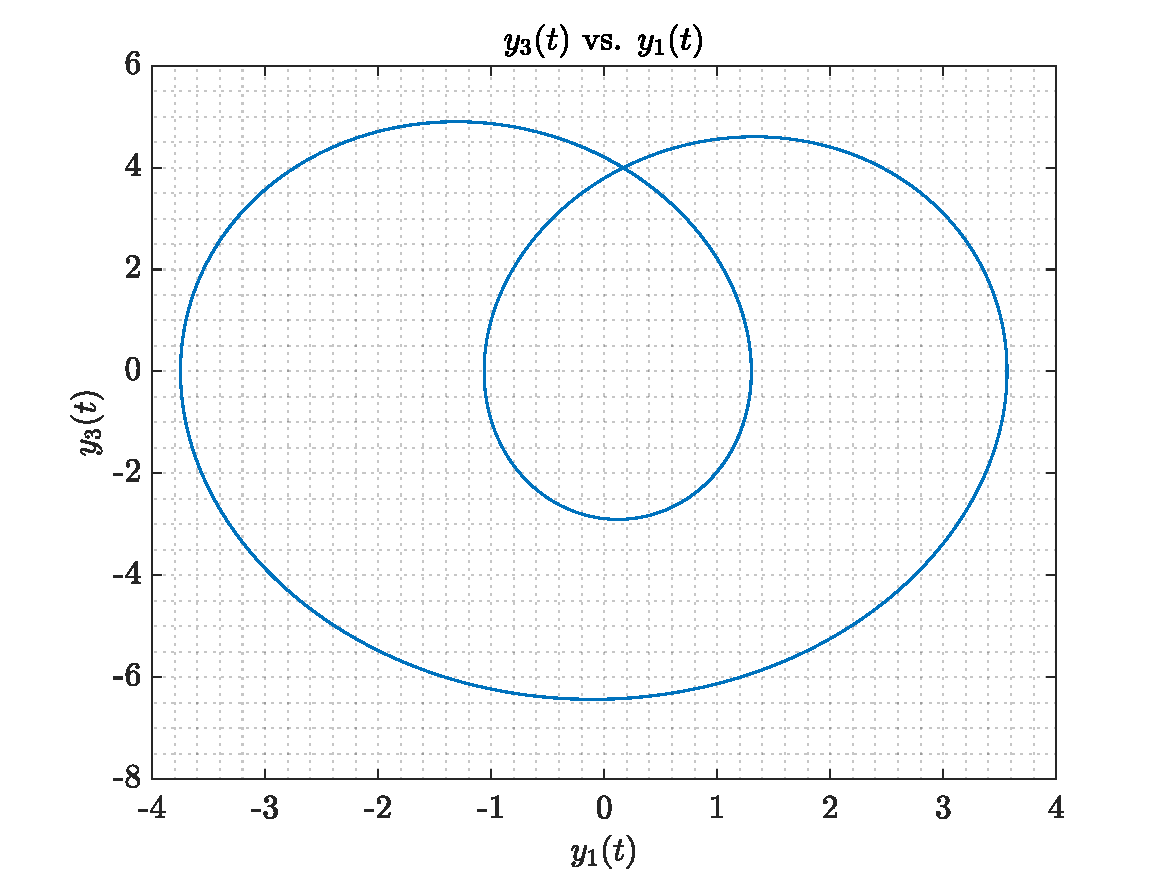
\includegraphics[height=0.3\textheight]{../Math.3341.Lab.14.ans/lab_14_figure_3.pdf}
  \caption{Expected result for System of ODEs}
  \label{fig:}
\end{figure}


